\chapter{The Laser: Stimulated Emission and Gaussian Beams}\label{ch:b2:laser}

A red dot on a lecture screen, the bar-code reader at the checkout,
the beam that reads a disc, welds a car body, carries the internet
under the oceans, corrects a cornea and measures the distance to the
Moon to a millimetre: every one of these is a \emph{\omterm{def:b2:laser:cavity}{laser}}, a source of
light unlike any flame or lamp. Its light is a single colour to a part
in a billion, stays in a beam of millimetres over a room, and can be
focused to a spot a few wavelengths wide, where its irradiance exceeds
that of the Sun's surface a million times. None of this comes from a
new kind of atom: it comes from a process Einstein identified in 1917
--- \emph{\omterm{def:b2:laser:processes}{stimulated emission}}, the emission of a photon identical to
one already present --- and from arranging matter so that this process
wins over \omterm{def:b2:laser:processes}{absorption}, then placing the amplifier between two mirrors
so that it feeds itself. This chapter builds the \omterm{def:b2:laser:cavity}{laser} in three steps:
how light and a population of atoms exchange energy (the \omterm{def:b2:laser:processes}{Einstein
coefficients}), when the exchange amplifies (\omterm{prop:b2:laser:gain}{population inversion} and
gain), and when the amplifier becomes an oscillator (the cavity, its
threshold and its modes). It ends with the shape of the beam that comes
out, the \omterm{prop:b2:laser:gaussian}{Gaussian beam}, whose \omterm{prop:b2:laser:gaussian}{waist} and \omterm{def:b2:maxwell-equations:operators}{divergence} decide what a \omterm{def:b2:laser:cavity}{laser}
can do at a distance and at a focus.

\begin{omfigure}
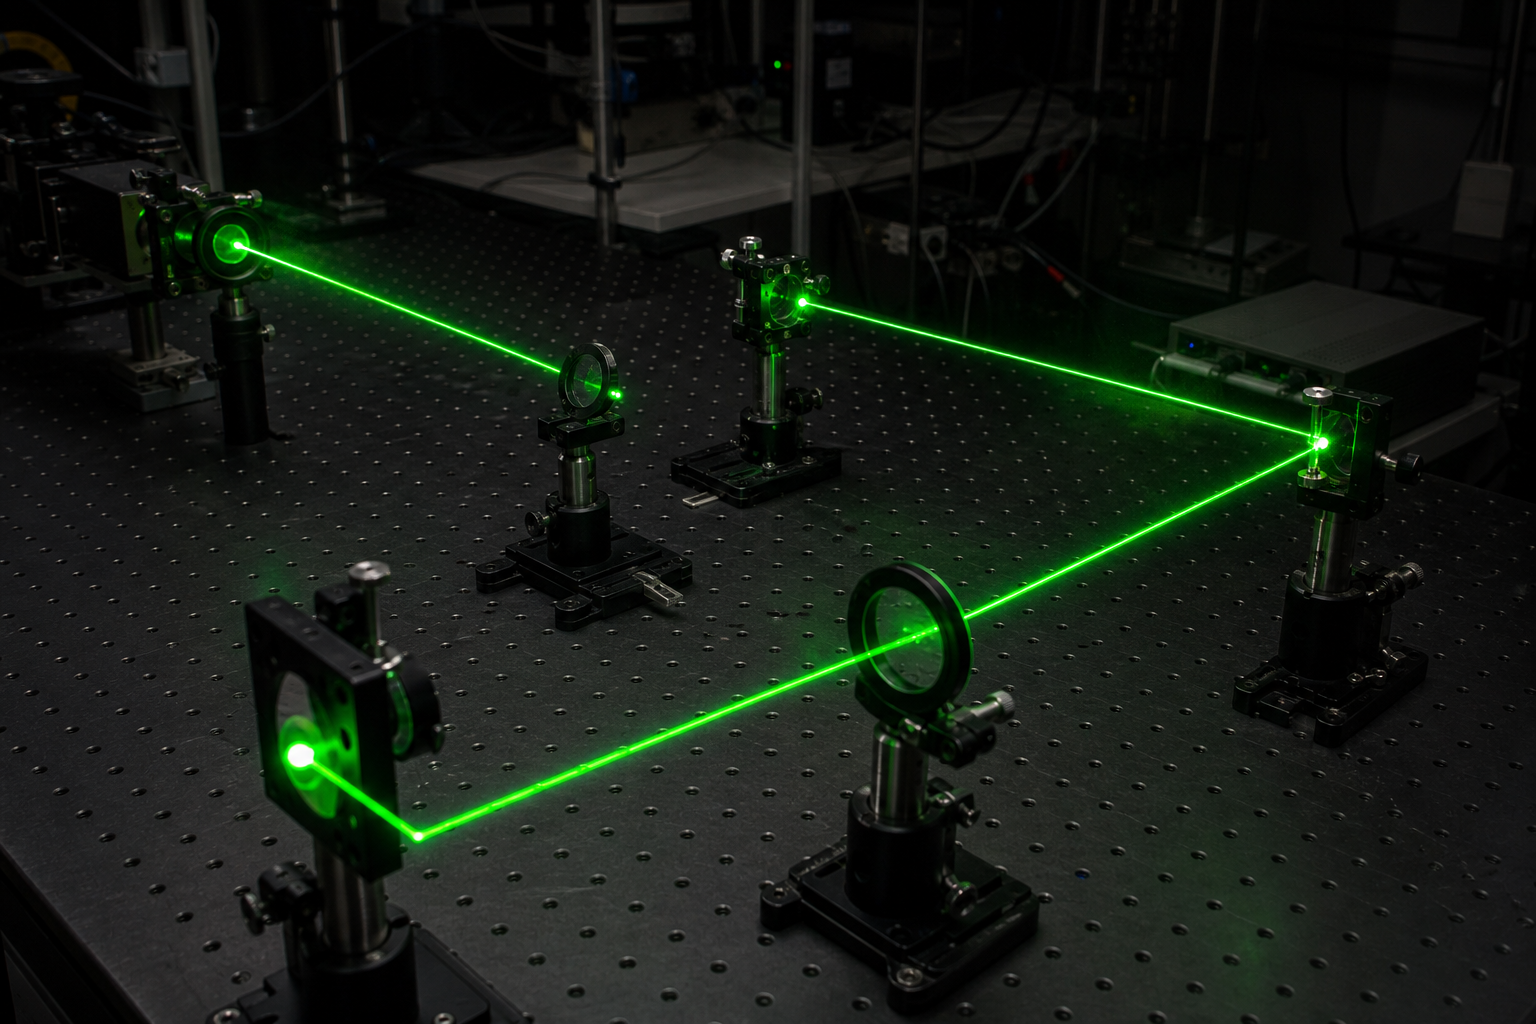
\includegraphics[width=0.58\linewidth]{images/book4/ai/b4-23-laser-optical-table.png}

{\small An optical table: \omterm{def:b2:laser:cavity}{laser}, mirrors, lenses and a beam that stays
a thin line across the whole room --- the directivity that no lamp can
give.}
\end{omfigure}

\section{Light and matter: the three processes}

\begin{definition}[Absorption, spontaneous and stimulated emission]\label{def:b2:laser:processes}
Consider atoms with two energy levels $E_1 < E_2$, populations (number
densities) $N_1$, $N_2$, and light of frequency $\nu$ with
$h\nu = E_2 - E_1$ and spectral energy density $u(\nu)$ (energy per unit
volume per unit frequency). Three processes exchange energy:
\begin{itemize}
\item \emph{absorption}\index{absorption (of light)}: an atom in
      $E_1$ absorbs a photon and rises to $E_2$, at the rate
      $B_{12}\,u(\nu)\,N_1$ per unit volume and time;
\item \emph{spontaneous emission}\index{spontaneous emission}: an atom
      in $E_2$ falls to $E_1$ on its own, emitting a photon in a random
      direction with a random phase, at the rate $A_{21}N_2$ ---
      $1/A_{21} = \tau$ is the lifetime of the level;
\item \emph{stimulated emission}\index{stimulated emission}: a photon
      of frequency $\nu$ passing an atom in $E_2$ induces it to fall,
      emitting a second photon \emph{identical} to the first (same
      frequency, direction, phase and polarization), at the rate
      $B_{21}\,u(\nu)\,N_2$.
\end{itemize}
$A_{21}$, $B_{12}$, $B_{21}$ are the \emph{Einstein
coefficients}\index{Einstein coefficients} of the transition.
\end{definition}

\begin{proposition}[Einstein relations]\label{prop:b2:laser:einstein}
For non-degenerate levels,
\[
B_{12} = B_{21} \equiv B, \qquad
\frac{A_{21}}{B_{21}} = \frac{8\pi h\nu^3}{c^3}.
\]
\omterm{def:b2:laser:processes}{Stimulated emission} and \omterm{def:b2:laser:processes}{absorption} have the same coefficient; the
spontaneous rate grows as $\nu^3$ relative to the stimulated rate.
\end{proposition}

\begin{proof}
Put the atoms in equilibrium with radiation at temperature $T$. Two
facts are borrowed from later chapters: the populations of two levels
at equilibrium are in the ratio $N_2/N_1 = \eu^{-h\nu/k_BT}$ (the
Boltzmann factor, \cref{ch:b2:boltzmann-factor}), and the equilibrium
radiation has the Planck spectral density
$u(\nu) = (8\pi h\nu^3/c^3)/(\eu^{h\nu/k_BT} - 1)$
(\cref{ch:b2:thermal-radiation}). At equilibrium the level populations
are steady: $B_{12}uN_1 = A_{21}N_2 + B_{21}uN_2$, hence
\[
u = \frac{A_{21}}{B_{12}\,N_1/N_2 - B_{21}}
  = \frac{A_{21}}{B_{12}\eu^{h\nu/k_BT} - B_{21}}.
\]
This must equal Planck's expression at every $T$: the $T \to \infty$
limit (where $u \to \infty$) forces $B_{12} = B_{21}$, and the
comparison then gives $A_{21}/B_{21} = 8\pi h\nu^3/c^3$. The
coefficients are properties of the atom, so the relations hold out of
equilibrium too.
\end{proof}

\begin{remark}[Why lamps do not amplify]\label{rem:b2:laser:lamps}
In a gas at \qty{300}{K}, for a visible transition ($h\nu \approx
\qty{2}{eV}$, $k_BT \approx \qty{0.025}{eV}$), $N_2/N_1 = \eu^{-80} \approx
10^{-35}$: essentially no atom is excited, and light is only absorbed. A
discharge or a flame populates $E_2$, but still with $N_2 < N_1$, and
every emitted photon is outnumbered by \omterm{def:b2:laser:processes}{absorptions}; moreover the ratio
of spontaneous to \omterm{def:b2:laser:processes}{stimulated emission} at equilibrium,
$A_{21}/(B_{21}u) = \eu^{h\nu/k_BT} - 1$, is astronomically large in the
visible --- a lamp's light is spontaneous: random phases, all
directions, the full width of the line. Only at radio and microwave
frequencies ($h\nu \ll k_BT$) does \omterm{def:b2:laser:processes}{stimulated emission} compete
naturally; the first device of this kind was indeed the maser, at
\qty{24}{GHz} (1954), before the optical \omterm{def:b2:laser:cavity}{laser} (1960).
\end{remark}

\begin{omfigure}
\begin{tikzpicture}[scale=0.9, >=stealth]
  \foreach \x/\t in {0/absorption, 3.6/spontaneous emission, 7.2/stimulated emission}{
    \draw[thick] (\x,0) -- ++(2,0) node[right, font=\scriptsize] {$E_1$};
    \draw[thick] (\x,1.6) -- ++(2,0) node[right, font=\scriptsize] {$E_2$};
    \node[font=\scriptsize, align=center] at (\x+1,-0.5) {\t};
  }
  % absorption
  \fill (1,0) circle (2pt);
  \draw[->, omDef, thick] (1,0.15) -- (1,1.45);
  \draw[->, omExo, thick, decorate, decoration={snake, amplitude=0.6mm, segment length=2mm}] (-0.6,0.8) -- (0.7,0.8);
  \node[font=\scriptsize, omExo] at (-0.5,1.15) {$h\nu$};
  % spontaneous
  \fill (4.6,1.6) circle (2pt);
  \draw[->, omDef, thick] (4.6,1.45) -- (4.6,0.15);
  \draw[->, omExo, thick, decorate, decoration={snake, amplitude=0.6mm, segment length=2mm}] (4.8,0.8) -- (6.2,1.3);
  % stimulated
  \fill (8.2,1.6) circle (2pt);
  \draw[->, omDef, thick] (8.2,1.45) -- (8.2,0.15);
  \draw[->, omExo, thick, decorate, decoration={snake, amplitude=0.6mm, segment length=2mm}] (6.6,0.8) -- (7.9,0.8);
  \draw[->, omExo, thick, decorate, decoration={snake, amplitude=0.6mm, segment length=2mm}] (8.5,0.95) -- (9.9,0.95);
  \draw[->, omExo, thick, decorate, decoration={snake, amplitude=0.6mm, segment length=2mm}] (8.5,0.65) -- (9.9,0.65);
  \node[font=\scriptsize, omExo] at (10.6,0.8) {$2h\nu$};
\end{tikzpicture}

{\small The three processes between two levels: \omterm{def:b2:laser:processes}{absorption} takes a
photon away; \omterm{def:b2:laser:processes}{spontaneous emission} adds a photon of random phase and
direction; \omterm{def:b2:laser:processes}{stimulated emission} adds a photon identical to the incident
one --- a copy.}
\end{omfigure}

\section{Amplification: population inversion and gain}

\begin{proposition}[Gain of a medium]\label{prop:b2:laser:gain}
A beam of intensity $I$ at the frequency $\nu$ crossing the medium
gains energy by \omterm{def:b2:laser:processes}{stimulated emission} and loses it by \omterm{def:b2:laser:processes}{absorption}
(\omterm{def:b2:laser:processes}{spontaneous emission} goes in all directions and hardly contributes to
the beam). Over a length $\dd z$,
\[
\dd I = \sigma\,(N_2 - N_1)\,I\,\dd z, \qquad
I(z) = I(0)\,\eu^{g z}, \qquad g = \sigma(N_2 - N_1),
\]
where $\sigma$ (an area, the \emph{cross-section}\index{cross-section
(of a transition)} of the transition, $\sigma \propto B\,h\nu/c$) measures
the strength of the transition. The medium \emph{amplifies} ($g > 0$)
only if
\[
N_2 > N_1 :
\]
a \emph{population inversion}\index{population inversion}. Without it
($N_2 < N_1$, the case of every medium at equilibrium) the beam is
absorbed.
\end{proposition}

\begin{proof}
Per unit volume and time, $B u (N_2 - N_1)$ transitions add (or remove)
a photon $h\nu$ to the beam; with $u = I/c$ (per unit frequency, over
the width of the line), the power gained per unit volume is
$B h\nu (N_2 - N_1) I/c$, and this is $\dd I/\dd z$; define $\sigma =
Bh\nu/c$ (times the line-shape factor).
\end{proof}

\begin{remark}[Why two levels cannot be inverted]\label{rem:b2:laser:twolevel}
Pump a two-level system as hard as you like with light at $\nu$: the
pump absorbs when $N_1 > N_2$ and stimulates emission when $N_2 > N_1$,
and the populations tend at best to equality, $N_2 = N_1$, where the
medium is transparent but gains nothing. An inversion needs at least
three levels: pump from the ground level to a short-lived level that
decays quickly into the upper \omterm{def:b2:laser:cavity}{laser} level, which is \emph{long-lived}
(metastable) and therefore stores population. In a
\emph{three-level}\index{three-level laser} scheme (ruby, the first
\omterm{def:b2:laser:cavity}{laser}) the lower \omterm{def:b2:laser:cavity}{laser} level is the ground state, so more than half
the atoms must be lifted before inversion: the pump is brutal. In a
\emph{four-level}\index{four-level laser} scheme (He--Ne, Nd:YAG, most
\omterm{def:b2:laser:cavity}{lasers}) the lower \omterm{def:b2:laser:cavity}{laser} level is an excited level that empties quickly
to the ground state; it is nearly empty at all times, and a small
population in the upper level is already an inversion --- the threshold
is low.
\end{remark}

\begin{omfigure}
\begin{tikzpicture}[scale=0.85, >=stealth]
  % three-level
  \draw[thick] (0,0) -- (2,0) node[right, font=\scriptsize] {$0$: ground};
  \draw[thick] (0,2.4) -- (2,2.4) node[right, font=\scriptsize] {$2$ (short-lived)};
  \draw[thick] (0,1.8) -- (2,1.8) node[right, font=\scriptsize] {$1$ (metastable)};
  \draw[->, omExo, thick] (0.5,0.05) -- (0.5,2.35) node[midway, left, font=\scriptsize] {pump};
  \draw[->, dashed] (1.0,2.35) -- (1.0,1.85);
  \draw[->, omDef, very thick] (1.5,1.75) -- (1.5,0.05) node[midway, right, font=\scriptsize] {laser};
  \node[font=\scriptsize] at (1.8,-0.6) {three levels (ruby)};
  % four-level
  \begin{scope}[xshift=7cm]
  \draw[thick] (0,0) -- (2,0) node[right, font=\scriptsize] {$0$: ground};
  \draw[thick] (0,2.4) -- (2,2.4) node[right, font=\scriptsize] {$3$ (short-lived)};
  \draw[thick] (0,1.9) -- (2,1.9) node[right, font=\scriptsize] {$2$ (metastable)};
  \draw[thick] (0,0.6) -- (2,0.6) node[right, font=\scriptsize] {$1$ (empties fast)};
  \draw[->, omExo, thick] (0.5,0.05) -- (0.5,2.35) node[midway, left, font=\scriptsize] {pump};
  \draw[->, dashed] (1.0,2.35) -- (1.0,1.95);
  \draw[->, omDef, very thick] (1.5,1.85) -- (1.5,0.65) node[midway, right, font=\scriptsize] {laser};
  \draw[->, dashed] (1.0,0.55) -- (1.0,0.05);
  \node[font=\scriptsize] at (1.8,-0.6) {four levels (He--Ne, Nd:YAG)};
  \end{scope}
\end{tikzpicture}

{\small Pumping schemes. Left: three levels --- the \omterm{def:b2:laser:cavity}{laser} transition
ends on the ground level, which must be more than half emptied. Right:
four levels --- the lower \omterm{def:b2:laser:cavity}{laser} level drains at once to the ground
state, so a small upper population is already an inversion.}
\end{omfigure}

\begin{proposition}[Saturation of the gain]\label{prop:b2:laser:saturation}
The inversion is maintained by a pump that supplies atoms to the upper
level at the rate $R$ per unit volume, against the decay $1/\tau$ and
the \omterm{def:b2:laser:processes}{stimulated emission} $\sigma I (N_2 - N_1)/h\nu$. In a four-level
medium ($N_1 \approx 0$) the steady state is
\[
N_2 = \frac{R\tau}{1 + I/I_{\text{s}}}, \qquad
g = \frac{g_0}{1 + I/I_{\text{s}}}, \qquad
I_{\text{s}} = \frac{h\nu}{\sigma\tau} :
\]
the \emph{small-signal gain} $g_0 = \sigma R\tau$ is reduced by the beam
itself once $I$ approaches the \emph{saturation
intensity}\index{saturation intensity} $I_{\text{s}}$ --- the amplifier
is nonlinear, and this nonlinearity is what will fix the power of the
\omterm{def:b2:laser:cavity}{laser}.
\end{proposition}

\begin{proof}
$\dd N_2/\dd t = R - N_2/\tau - \sigma I N_2/h\nu = 0$.
\end{proof}

\section{The oscillator: cavity, threshold and modes}

\begin{definition}[Laser cavity]\label{def:b2:laser:cavity}
A \emph{laser}\index{laser} is an amplifying medium of length $\ell$
placed between two mirrors (reflectances $R_1$, $R_2$) a distance $L$
apart: a Fabry--Pérot cavity (\cref{ch:b2:gratings}). One mirror, the
\emph{output coupler}, is partly transmitting ($T_2 = 1 - R_2$ of a few
per cent) and lets the beam out. Light that goes round the cavity is
amplified twice by the medium and attenuated by the mirrors and by the
other losses (scattering, \omterm{def:b2:laser:processes}{absorption}, \omterm{def:b2:diffraction:huygens}{diffraction}).
\end{definition}

\begin{theorem}[Oscillation condition]\label{thm:b2:laser:threshold}
A wave of complex amplitude $\underline s$ reproduces itself after one
round trip if
\[
\underline s\,\cdot\, \eu^{g\ell}\sqrt{R_1}\,\eu^{g\ell}\sqrt{R_2}\,
\eu^{-\alpha\cdot 2L}\,\eu^{2\iu kL} = \underline s
\]
($\alpha$: the other losses per unit length). Hence two conditions.
\begin{itemize}
\item \emph{Amplitude}: $R_1R_2\,\eu^{2(g\ell - \alpha L)} \ge 1$, i.e. the
      gain must reach the \emph{threshold}\index{threshold (laser)}
      \[
      g_{\text{th}} = \frac{1}{\ell}\Big(\alpha L - \tfrac12\ln(R_1R_2)\Big)
      \approx \frac{1}{2\ell}\,(T_2 + \text{losses per round trip}) ;
      \]
\item \emph{Phase}: $2kL = 2\pi p$, i.e. $\nu_p = p\,c/2L$ --- the \omterm{def:b2:laser:cavity}{laser}
      oscillates only on the \emph{longitudinal modes}\index{longitudinal
      modes} of the cavity, spaced by $c/2L$, and among them only on
      those lying under the gain curve where $g(\nu) \ge g_{\text{th}}$.
\end{itemize}
\end{theorem}

\begin{proof}
Amplitude and phase of the round-trip factor must both be trivial; the
approximation uses $-\ln R \approx 1 - R = T$ for $T \ll 1$.
\end{proof}

\begin{proposition}[Steady state above threshold]\label{prop:b2:laser:steady}
Starting from the \omterm{def:b2:laser:processes}{spontaneous emission} of a single atom, any mode for
which $g_0 > g_{\text{th}}$ grows exponentially, round trip after round
trip; as its intensity grows, the gain saturates
(\cref{prop:b2:laser:saturation}) until it equals exactly the losses:
\[
g(I) = g_{\text{th}} \quad\Longrightarrow\quad
I_{\text{cavity}} = I_{\text{s}}\Big(\frac{g_0}{g_{\text{th}}} - 1\Big),
\qquad P_{\text{out}} = T_2\,I_{\text{cavity}}\,A .
\]
The gain \emph{clamps} to the threshold value; every additional atom
pumped above threshold becomes an output photon, so the output power
grows linearly with the pump above the threshold pump.
\end{proposition}

\begin{remark}[The laser is a feedback oscillator]\label{rem:b2:laser:feedback}
Compare with the \omterm{prop:b2:feedback-oscillators:wien}{Wien-bridge oscillator} of
\cref{ch:b2:feedback-oscillators}: an amplifier (the inverted medium),
a frequency-selective \omterm{def:b2:feedback-oscillators:loop}{feedback} (the cavity, passing only its modes),
a start-up condition (\omterm{def:b2:feedback-oscillators:loop}{loop gain} $> 1$, i.e. $g_0 > g_{\text{th}}$),
start-up from noise (here \omterm{def:b2:laser:processes}{spontaneous emission}), and an amplitude fixed
by the nonlinearity of the amplifier (gain saturation). The \omterm{def:b2:laser:cavity}{laser} is
the optical member of the family.
\end{remark}

\begin{omfigure}
\begin{tikzpicture}
  \begin{axis}[omaxis, width=8.2cm, height=4.6cm, xmin=-2.4, xmax=2.4, ymin=0, ymax=1.25,
    xlabel={$(\nu - \nu_0)/\Delta\nu$}, ylabel={$g(\nu)$}, ytick=\empty,
    xtick={-2,-1,0,1,2}, clip=false]
    \addplot[omDef, thick, domain=-2.4:2.4, samples=120] {exp(-2.77*x*x)};
    \addplot[omExo, thick, dashed, domain=-2.4:2.4] {0.45};
    \node[font=\scriptsize, omExo, anchor=west] at (axis cs:1.6,0.55) {$g_{\text{th}}$};
    \draw[gray!70] (axis cs:-1.75,0) -- (axis cs:-1.75,0.12);
    \draw[gray!70] (axis cs:-1.4,0) -- (axis cs:-1.4,0.12);
    \draw[gray!70] (axis cs:-1.05,0) -- (axis cs:-1.05,0.12);
    \draw[gray!70] (axis cs:-0.7,0) -- (axis cs:-0.7,0.12);
    \draw[gray!70] (axis cs:0.7,0) -- (axis cs:0.7,0.12);
    \draw[gray!70] (axis cs:1.05,0) -- (axis cs:1.05,0.12);
    \draw[gray!70] (axis cs:1.4,0) -- (axis cs:1.4,0.12);
    \draw[gray!70] (axis cs:1.75,0) -- (axis cs:1.75,0.12);
    \draw[omThm, very thick] (axis cs:-0.35,0) -- (axis cs:-0.35,0.712);
    \draw[omThm, very thick] (axis cs:0,0) -- (axis cs:0,1.000);
    \draw[omThm, very thick] (axis cs:0.35,0) -- (axis cs:0.35,0.712);
    \node[font=\scriptsize, anchor=south] at (axis cs:-1.4,0.14) {$c/2L$};
    \draw[<->, thin] (axis cs:-1.75,0.12) -- (axis cs:-1.05,0.12);
  \end{axis}
\end{tikzpicture}

{\small The gain curve of the medium (width $\Delta\nu$), the threshold
set by the losses, and the comb of cavity modes spaced $c/2L$: only the
modes under the curve and above threshold (heavy) oscillate.}
\end{omfigure}

\begin{example}[The helium--neon laser]\label{ex:b2:laser:hene}
A glass tube \qty{30}{cm} long, bore \qty{1}{mm}, holding helium and
neon at about a thousandth of an atmosphere, crossed by a discharge of
a few milliamperes. Electrons excite helium to a metastable level at
\qty{20.6}{eV}, which hands its energy by collision to a neon level at
almost exactly the same height; from there neon decays to a lower level
(emptying fast to the ground state --- four-level) by emitting at
\qty{632.8}{nm}. The small-signal gain is tiny, a few per cent per
pass, so the mirrors must be excellent ($R_1 = 0.999$, $R_2 = 0.99$)
and the tube clean; the gain line is Doppler-broadened to
$\Delta\nu \approx \qty{1.5}{GHz}$, the modes are $c/2L = \qty{500}{MHz}$
apart, so two or three modes oscillate at once. Output \qty{1}{mW} for
several watts of discharge: efficiency $10^{-4}$; but a wavelength
defined to $10^{-6}$ and a beam that stays \qty{1}{mm} wide across the
laboratory.
\end{example}

\section{The Gaussian beam}

\begin{proposition}[Gaussian beam]\label{prop:b2:laser:gaussian}
The beam that a stable cavity with curved mirrors emits is (in the
fundamental transverse mode) a \emph{Gaussian beam}\index{Gaussian
beam}: at the distance $z$ from its narrowest section (the
\emph{waist}\index{waist (of a beam)}, radius $w_0$) the intensity
profile is
\[
I(r,z) = \frac{2P}{\pi w(z)^2}\,\exp\Big(-\frac{2r^2}{w(z)^2}\Big),
\qquad
w(z) = w_0\sqrt{1 + \Big(\frac{z}{z_{\text{R}}}\Big)^2},
\qquad
z_{\text{R}} = \frac{\pi w_0^2}{\lambda},
\]
where $P$ is the total power and $z_{\text{R}}$ the \emph{Rayleigh
length}\index{Rayleigh length}: over $\pm z_{\text{R}}$ the beam stays
within $\sqrt2$ of its \omterm{prop:b2:laser:gaussian}{waist}, and far beyond it spreads with the
half-angle
\[
\theta = \frac{\lambda}{\pi w_0} .
\]
The beam is a solution of the \omterm{thm:b2:waves-on-strings:equation}{wave equation} in the paraxial
approximation; we admit its form and use it. Its \omterm{def:b2:scalar-light-model:path}{wavefronts} are plane at
the \omterm{prop:b2:laser:gaussian}{waist} and spherical far away.
\end{proposition}

\begin{proof}
Admitted at this level (the calculation is the Fourier-optics
propagation of a Gaussian aperture distribution); its key property is
the one \omterm{def:b2:diffraction:huygens}{diffraction} already gave in \cref{ch:b2:diffraction}: an
aperture of size $w_0$ spreads over $\lambda/w_0$, here with the exact
factor $1/\pi$.
\end{proof}

\begin{omfigure}
\begin{tikzpicture}
  \begin{axis}[omaxis, width=9cm, height=4.6cm, xmin=-3.2, xmax=3.2, ymin=-3.4, ymax=3.4,
    xlabel={$z/z_{\text{R}}$}, ylabel={$r/w_0$}, clip=false, xtick={-3,-2,-1,0,1,2,3}, ytick={-2,-1,1,2}]
    \addplot[omDef, thick, domain=-3.2:3.2, samples=100] {sqrt(1+x*x)};
    \addplot[omDef, thick, domain=-3.2:3.2, samples=100] {-sqrt(1+x*x)};
    \addplot[omExo, dashed, domain=-3.2:3.2] {x};
    \addplot[omExo, dashed, domain=-3.2:3.2] {-x};
    \draw[<->, thin] (axis cs:0.3,-1.04) -- (axis cs:0.3,1.04) node[pos=0.25, right, font=\scriptsize] {$2w_0$};
    \node[font=\scriptsize, omExo, anchor=north west] at (axis cs:0.8,3.5) {$\theta = \lambda/\pi w_0$};
  \end{axis}
\end{tikzpicture}

{\small A \omterm{prop:b2:laser:gaussian}{Gaussian beam}: the radius $w(z)$ is a hyperbola --- nearly
constant within the \omterm{prop:b2:laser:gaussian}{Rayleigh length}, then a cone of half-angle
$\lambda/\pi w_0$. A smaller \omterm{prop:b2:laser:gaussian}{waist} means a shorter \omterm{prop:b2:laser:gaussian}{Rayleigh length} and a
wider cone.}
\end{omfigure}

\begin{proposition}[Focusing and expanding a beam]\label{prop:b2:laser:focus}
A \omterm{prop:b2:laser:gaussian}{Gaussian beam} of radius $w$ (much larger than its far-field would
have at the lens, i.e. nearly collimated) falling on a lens of focal
length $f$ is focused to a \omterm{prop:b2:laser:gaussian}{waist}
\[
w_0' = \frac{\lambda f}{\pi w}
\]
at the focus, with \omterm{prop:b2:laser:gaussian}{Rayleigh length} $\pi w_0'^2/\lambda$. The peak
irradiance there is $2P/\pi w_0'^2$. Conversely an afocal telescope of
magnification $M$ turns a beam of radius $w$ into one of radius $Mw$
whose \omterm{def:b2:maxwell-equations:operators}{divergence} is $M$ times smaller: to send a beam far, first make
it wide.
\end{proposition}

\begin{proof}
The lens converts the plane \omterm{def:b2:scalar-light-model:path}{wavefront} into a sphere converging at $f$;
the \omterm{def:b2:diffraction:huygens}{diffraction} of an aperture of radius $w$ gives the angular spread
$\lambda/\pi w$, hence the focal spot $f\lambda/\pi w$ --- consistent with
$\theta = \lambda/\pi w_0'$ read backwards.
\end{proof}

\begin{example}[Cutting, reading, pointing]\label{ex:b2:laser:focus}
A \qty{1}{kW} carbon-dioxide \omterm{def:b2:laser:cavity}{laser} at \qty{10.6}{\micro m}, beam radius
\qty{10}{mm}, focused by $f = \qty{100}{mm}$: $w_0' = \qty{34}{\micro m}$,
peak irradiance $2P/\pi w_0'^2 = \qty{5e11}{W/m^2}$ --- steel boils.
A \qty{1}{mW} pointer, $w_0 = \qty{0.5}{mm}$ at \qty{633}{nm}: $\theta =
\qty{0.4}{mrad}$, a \qty{4}{cm} spot at \qty{50}{m}, an irradiance of
\qty{2.5}{kW/m^2} at the exit --- above sunlight, which is why even a
milliwatt must never enter an eye: the eye's lens would focus it to a
\qty{10}{\micro m} spot on the retina at millions of watts per square
metre. A disc reader at \qty{650}{nm} with a lens of \omterm{prop:b2:guided-waves:fibre}{numerical aperture}
$0.6$ focuses to about $\lambda/2\mathrm{NA} \approx \qty{0.5}{\micro m}$,
the size of a pit.
\end{example}

\begin{remark}[What makes laser light special]\label{rem:b2:laser:special}
\emph{Directivity}: one transverse mode, \omterm{def:b2:maxwell-equations:operators}{divergence} at the \omterm{def:b2:diffraction:huygens}{diffraction}
limit. \emph{Monochromaticity}: one or a few cavity modes, each
narrower than a megahertz --- \omterm{prop:b2:scalar-light-model:coherence}{coherence lengths} of metres to kilometres
(\cref{ch:b2:scalar-light-model}). \emph{\omterm{prop:b2:two-wave-interference:spatial}{Spatial coherence}}: the whole
beam is one wave, so it interferes with itself anywhere (holography,
interferometry). \emph{Brightness}: a milliwatt in a diffraction-limited
beam outshines the Sun per unit solid angle and bandwidth. \emph{Power}
in pulses: a joule in a nanosecond is a gigawatt, in a femtosecond a
petawatt. And, since the beam is an oscillator's output, it can be
modulated at gigahertz --- the carrier of the \omterm{prop:b2:guided-waves:fibre}{optical fibre}
(\cref{ch:b2:guided-waves}).
\end{remark}

\begin{method}[Laser estimates]\label{meth:b2:laser:method}
(1) Photon energy $h\nu = hc/\lambda$ and the photon rate $P/h\nu$.
(2) Threshold: $g_{\text{th}}\ell \approx \tfrac12(T_2 + \text{losses})$;
compare with the small-signal gain $g_0\ell$ of the medium.
(3) Modes: $c/2L$ against the gain width; count the oscillating modes.
(4) Power: gain clamps at threshold; output $\propto$ (pump $-$
threshold pump). (5) Beam: $z_{\text{R}} = \pi w_0^2/\lambda$, $\theta =
\lambda/\pi w_0$, focal spot $\lambda f/\pi w$, peak irradiance
$2P/\pi w_0^2$. (6) Safety: compare the retinal irradiance with the
Sun's.
\end{method}

\section{Exercises}

\begin{exercise}[$\star$]\label{exo:b2:laser:1}
A He--Ne \omterm{def:b2:laser:cavity}{laser} emits \qty{1}{mW} at \qty{632.8}{nm}. Frequency, photon
energy in joules and electronvolts, photons per second. Cavity
\qty{30}{cm}: mode spacing; how many modes fit under a gain curve
\qty{1.5}{GHz} wide?
\end{exercise}

\begin{exercise}[$\star$]\label{exo:b2:laser:2}
Two levels \qty{2}{eV} apart at \qty{300}{K}: ratio $N_2/N_1$ (use
$k_BT = \qty{0.025}{eV}$). At what temperature would the populations be
equal? Show that an inversion corresponds to a formally \emph{negative}
temperature in the Boltzmann ratio. Same ratio for a microwave
transition at \qty{24}{GHz}.
\end{exercise}

\begin{exercise}[$\star$]\label{exo:b2:laser:3}
\omterm{prop:b2:laser:gaussian}{Gaussian beam}, $w_0 = \qty{0.5}{mm}$, $\lambda = \qty{633}{nm}$: \omterm{prop:b2:laser:gaussian}{Rayleigh
length}, \omterm{def:b2:maxwell-equations:operators}{divergence}, radius after \qty{100}{m} and at the Moon
(\qty{3.8e8}{m}). Same beam after a $\times 20$ expander.
\end{exercise}

\begin{exercise}[$\star$]\label{exo:b2:laser:4}
Cavity with $R_1 = 1$, $R_2 = 0.98$, medium \qty{20}{cm} long, other
losses $0.5\%$ per pass. Threshold gain coefficient. The medium's
small-signal gain is \qty{0.2}{m^{-1}}: does it lase? With
$R_2 = 0.90$?
\end{exercise}

\begin{exercise}[$\star\star$]\label{exo:b2:laser:5}
\emph{Einstein relations.} (a) Write the balance of a two-level
population in equilibrium with radiation $u(\nu)$ and derive the two
relations from Planck's law (given). (b) Compute
$A_{21}/B_{21}u = \eu^{h\nu/k_BT} - 1$ at \qty{300}{K} for
$\lambda = \qty{600}{nm}$ and for $\lambda = \qty{1}{cm}$. (c) Why were
masers invented before \omterm{def:b2:laser:cavity}{lasers}? (d) A level's lifetime is
$\tau = 1/A_{21}$; if $\tau = \qty{10}{ns}$ at \qty{600}{nm}, what is
$\tau$ for a transition of the same $B$ at \qty{6}{\micro m}?
\end{exercise}

\begin{exercise}[$\star\star$]\label{exo:b2:laser:6}
\emph{Saturation and output power.} Four-level medium, $\sigma =
\qty{3e-17}{m^2}$, $\tau = \qty{100}{ns}$, $\lambda = \qty{633}{nm}$.
(a) \omterm{prop:b2:laser:saturation}{Saturation intensity}. (b) Pump rate $R$ for a small-signal gain
$g_0 = \qty{0.1}{m^{-1}}$. (c) The cavity's threshold is
$g_{\text{th}} = \qty{0.02}{m^{-1}}$: intracavity intensity in steady
state; output through $T_2 = 1\%$ from a beam of area \qty{1}{mm^2}.
(d) Show that the output power is linear in $R$ above threshold.
\end{exercise}

\begin{exercise}[$\star\star$]\label{exo:b2:laser:7}
\emph{Modes and stability.} (a) Cavity length for single-mode operation
under a \qty{1.5}{GHz} gain curve. (b) A \qty{30}{cm} cavity expands
by \qty{1}{\micro m}: shift of a mode's frequency, compared with the
mode spacing and the gain width. (c) Why do commercial stabilised He--Ne
\omterm{def:b2:laser:cavity}{lasers} lock the tube length by heating it? (d) The mode's own width is
a few kilohertz: \omterm{prop:b2:scalar-light-model:coherence}{coherence length}?
\end{exercise}

\begin{exercise}[$\star\star$]\label{exo:b2:laser:8}
\emph{Focusing.} (a) Beam $w = \qty{1}{mm}$, $\lambda = \qty{633}{nm}$,
$f = \qty{50}{mm}$: \omterm{prop:b2:laser:gaussian}{waist}, \omterm{prop:b2:laser:gaussian}{Rayleigh length}, peak irradiance for
\qty{1}{mW}. (b) The same beam into an eye (focal \qty{17}{mm}):
retinal spot and irradiance; compare with the Sun's image
(\qty{1}{kW/m^2} through a \qty{3}{mm} pupil into a \qty{0.15}{mm}
image). (c) Why is a \qty{5}{mW} green pointer more dangerous than a
\qty{100}{W} bulb? (d) Depth of focus of the \qty{50}{mm} lens.
\end{exercise}

\begin{exercise}[$\star\star$]\label{exo:b2:laser:9}
\emph{Three versus four levels.} Ruby: $N = \qty{1.6e25}{m^{-3}}$
chromium ions, upper-level lifetime \qty{3}{ms}, $\lambda =
\qty{694}{nm}$. (a) Minimum pump power per unit volume to hold half the
ions in the upper level. (b) For a \qty{1}{cm^3} rod. (c) A four-level
medium needs only $\Delta N = \qty{1e22}{m^{-3}}$ with $\tau =
\qty{230}{\micro s}$ at \qty{1064}{nm}: pump power per unit volume. (d) Comment on the
flash lamp of the ruby \omterm{def:b2:laser:cavity}{laser} versus the diode pumping of a Nd:YAG.
\end{exercise}

\begin{exercise}[$\star\star\star$]\label{exo:b2:laser:10}
\emph{The \omterm{def:b2:laser:cavity}{laser} diode.} The emitting region of a diode \omterm{def:b2:laser:cavity}{laser} is about
\qty{3}{\micro m} by \qty{1}{\micro m}, $\lambda = \qty{780}{nm}$. (a)
\omterm{def:b2:maxwell-equations:operators}{Divergence} half-angles in the two directions. (b) Which direction
diverges more, and why is the beam elliptical? (c) A lens of $f =
\qty{5}{mm}$ collimates it: beam sizes in the two directions. (d) How
can the ellipse be made round (two ideas)?
\end{exercise}

\begin{exercise}[$\star\star\star$]\label{exo:b2:laser:11}
\emph{Start-up.} (a) Write the round-trip amplitude condition with a
net gain $G = \eu^{2(g_0 - g_{\text{th}})\ell} = 1.04$ per round trip
and a round-trip time $2L/c$ with $L = \qty{30}{cm}$. (b) From one
spontaneous photon to the steady state of \qty{100}{mW} intracavity
(photon number in the cavity?), how many round trips and how long?
(c) What limits the growth, and what happens to a mode whose
$g_0 < g_{\text{th}}$? (d) In a multimode \omterm{def:b2:laser:cavity}{laser} the modes compete for
the same atoms: explain mode hopping.
\end{exercise}

\begin{exercise}[$\star\star\star$]\label{exo:b2:laser:12}
\emph{Lunar ranging.} Pulses of \qty{100}{mJ} at \qty{532}{nm},
\qty{100}{ps} long, sent through a \qty{1}{m} telescope ($w_0 =
\qty{0.5}{m}$). (a) Photons per pulse, peak power. (b) \omterm{def:b2:diffraction:huygens}{Diffraction}
\omterm{def:b2:maxwell-equations:operators}{divergence} and spot radius on the Moon (\qty{3.8e8}{m}); the atmosphere
spreads the beam to \qty{1}{''} instead: spot radius. (c) A reflector
array of \qty{0.1}{m^2} on the Moon returns the light with its own
\omterm{def:b2:diffraction:huygens}{diffraction} ($\lambda/d$ with $d = \qty{4}{cm}$ corner cubes): spot on
Earth, fraction caught by the telescope, photons per pulse detected.
(d) Timing to \qty{100}{ps}: distance precision per pulse, and after
$10^4$ pulses.
\end{exercise}

\begin{omfigure}
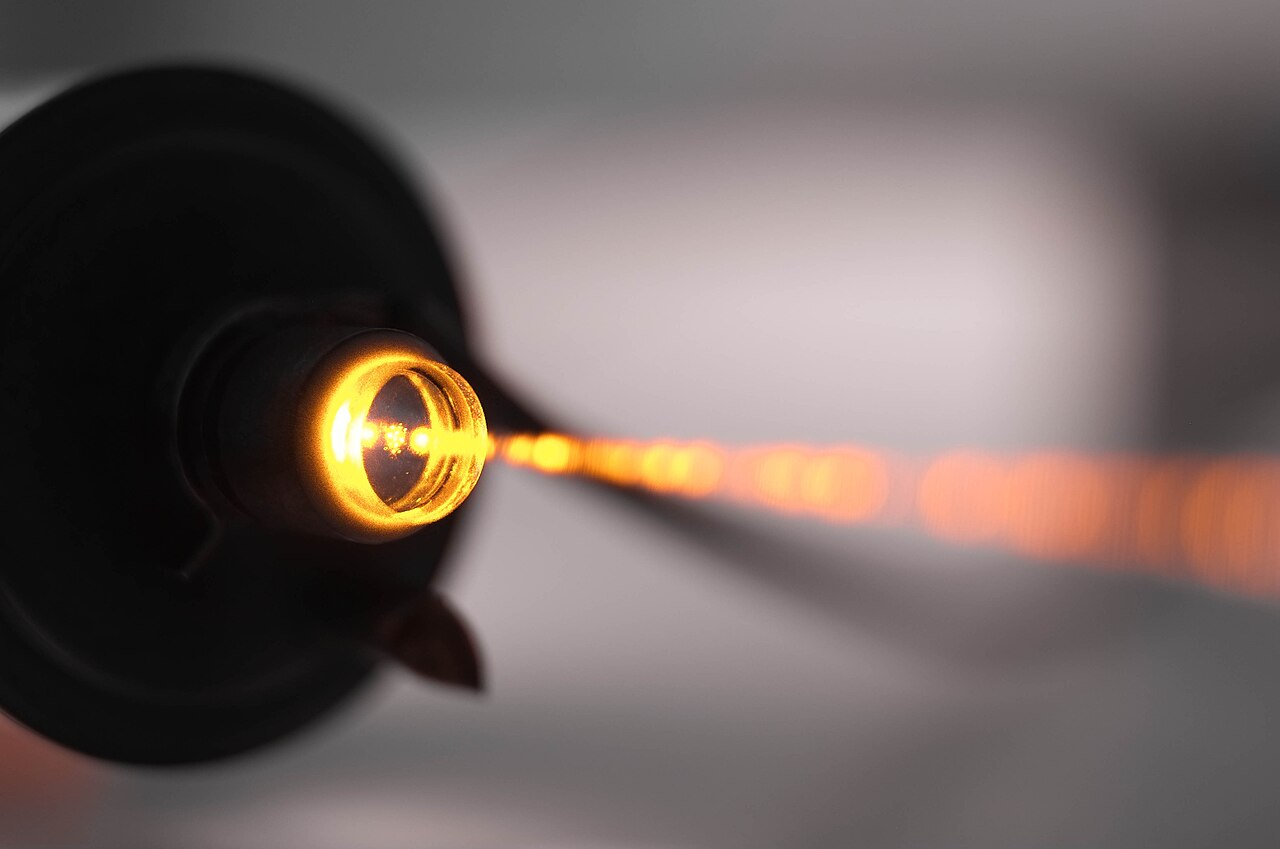
\includegraphics[width=0.58\linewidth]{images/book4/hene-laser-594nm.jpg}

{\small A helium--neon \omterm{def:b2:laser:cavity}{laser} tube emitting on its yellow line at \qty{594}{nm}: the glow of the discharge inside the tube, and the beam leaving through the output mirror. Photo: Telementor, CC~BY~4.0.}
\end{omfigure}

\section{Problem: A helium--neon laser, from the tube to the Moon}

\begin{problem}[{Weekend problem --- a laser built, characterised and
used}]\label{pb:b2:laser:1}
The \omterm{def:b2:laser:cavity}{laser} on the bench: glass tube $L = \qty{30}{cm}$, bore diameter
\qty{1}{mm}, helium--neon mixture, discharge \qty{5}{mA} under
\qty{1.5}{kV}; mirrors $R_1 = 0.999$, $R_2 = 0.99$; wavelength
\qty{632.8}{nm}; output \qty{1}{mW}. Data: the He metastable level lies
at \qty{20.61}{eV}, the Ne upper \omterm{def:b2:laser:cavity}{laser} level at \qty{20.66}{eV} with
lifetime \qty{100}{ns}, the lower \omterm{def:b2:laser:cavity}{laser} level at \qty{18.70}{eV} with
lifetime \qty{10}{ns}; gas temperature \qty{400}{K}; neon molar mass
\qty{20}{g/mol}; \omterm{prop:b2:laser:gain}{cross-section} $\sigma = \qty{3e-17}{m^2}$; $h =
\qty{6.63e-34}{J.s}$, $k_B = \qty{1.38e-23}{J/K}$, $k_BT$ at \qty{400}{K}
$= \qty{0.0345}{eV}$.

\textbf{Part I --- The medium.}
\begin{enumerate}
  \item Photon energy and frequency of the \omterm{def:b2:laser:cavity}{laser} line.
  \item The He and Ne levels differ by \qty{0.05}{eV}: compare with
        $k_BT$ and explain why the collision transfer He $\to$ Ne is
        efficient.
  \item Boltzmann ratio of the Ne upper level to the ground state at
        \qty{400}{K} without the discharge: comment.
  \item Explain, from the two lifetimes, why an inversion between the
        Ne levels is easy to maintain once the upper level is fed.
  \item Doppler width of the line: the most probable speed of neon at
        \qty{400}{K} and $\Delta\nu \approx \nu\,v/c$ in order of
        magnitude (precisely $\Delta\nu = 2\nu\sqrt{2k_BT\ln2/Mc^2}$).
  \item With $\Delta N = N_2 - N_1 = \qty{3e15}{m^{-3}}$: small-signal
        gain coefficient and gain per pass over \qty{30}{cm}.
\end{enumerate}

\textbf{Part II --- The cavity.}
\begin{enumerate}[resume]
  \item Threshold gain coefficient; margin with respect to question 6.
  \item Mode spacing; number of modes that can oscillate.
  \item Intracavity power and intracavity irradiance in the bore.
  \item What fixes the gain in steady state, and where does the extra
        pump energy go?
  \item Electrical power in and optical power out: efficiency; two
        reasons why it is so low.
  \item Start-up: net gain per round trip $2(g_0 - g_{\text{th}})L$,
        number of photons in the cavity at steady state, number of
        round trips from one photon, and the start-up time.
  \item The tube warms and lengthens by \qty{1}{\micro m}: frequency
        shift of a mode; consequence for a single-mode \omterm{def:b2:laser:cavity}{laser}.
  \item The tube is closed by windows at Brewster's angle: what does
        this do to the polarization of the output, and why does it not
        add loss?
\end{enumerate}

\textbf{Part III --- The beam.}
\begin{enumerate}[resume]
  \item The cavity produces a \omterm{prop:b2:laser:gaussian}{waist} $w_0 = \qty{0.3}{mm}$: \omterm{prop:b2:laser:gaussian}{Rayleigh
        length}, \omterm{def:b2:maxwell-equations:operators}{divergence}, beam diameter \qty{10}{m} away.
  \item Peak irradiance at the exit; compare with sunlight
        (\qty{1}{kW/m^2}).
  \item A lens of $f = \qty{50}{mm}$: \omterm{prop:b2:laser:gaussian}{waist} and peak irradiance at the
        focus.
  \item The beam enters an eye (focal length \qty{17}{mm}): retinal spot
        and irradiance; why a blink is not too slow for \qty{1}{mW},
        and what ``class 2'' means.
  \item A $\times 10$ beam expander: new \omterm{def:b2:maxwell-equations:operators}{divergence} and spot diameter
        at \qty{1}{km}.
  \item \omterm{prop:b2:scalar-light-model:coherence}{Coherence length} if the \omterm{def:b2:laser:cavity}{laser} runs on a single mode of width
        \qty{1}{MHz}; if it runs on three modes spanning \qty{1}{GHz}.
\end{enumerate}

\textbf{Part IV --- To the Moon.}
A ranging station fires \qty{100}{mJ} pulses of \qty{100}{ps} at
\qty{532}{nm} through a \qty{1}{m} telescope; the atmosphere spreads
the outgoing beam to \qty{1}{''} ($\qty{4.8e-6}{rad}$).
\begin{enumerate}[resume]
  \item Photons per pulse and peak power.
  \item Spot radius on the Moon (\qty{3.8e8}{m}); compare with the
        diffraction-limited spot.
  \item A reflector array of \qty{0.1}{m^2} intercepts what fraction of
        the pulse, how many photons?
  \item The array's \qty{4}{cm} corner cubes return the light with the
        spread $\lambda/d$: spot radius on Earth, fraction caught by the
        telescope, photons detected per pulse (take an overall optical
        efficiency of $0.1$).
  \item The round-trip time is about \qty{2.56}{s}, measured to
        \qty{100}{ps}: distance precision per pulse; after $10^4$
        returns; compare with the \qty{3.8}{cm} per year at which the
        Moon recedes.
\end{enumerate}
\end{problem}
